\documentclass[]{article}
\usepackage{lmodern}
\usepackage{amssymb,amsmath}
\usepackage{ifxetex,ifluatex}
\usepackage{fixltx2e} % provides \textsubscript
\ifnum 0\ifxetex 1\fi\ifluatex 1\fi=0 % if pdftex
  \usepackage[T1]{fontenc}
  \usepackage[utf8]{inputenc}
\else % if luatex or xelatex
  \ifxetex
    \usepackage{mathspec}
    \usepackage{xltxtra,xunicode}
  \else
    \usepackage{fontspec}
  \fi
  \defaultfontfeatures{Mapping=tex-text,Scale=MatchLowercase}
  \newcommand{\euro}{€}
\fi
% use upquote if available, for straight quotes in verbatim environments
\IfFileExists{upquote.sty}{\usepackage{upquote}}{}
% use microtype if available
\IfFileExists{microtype.sty}{%
\usepackage{microtype}
\UseMicrotypeSet[protrusion]{basicmath} % disable protrusion for tt fonts
}{}
\usepackage[margin=1in]{geometry}
\usepackage{color}
\usepackage{fancyvrb}
\newcommand{\VerbBar}{|}
\newcommand{\VERB}{\Verb[commandchars=\\\{\}]}
\DefineVerbatimEnvironment{Highlighting}{Verbatim}{commandchars=\\\{\}}
% Add ',fontsize=\small' for more characters per line
\usepackage{framed}
\definecolor{shadecolor}{RGB}{248,248,248}
\newenvironment{Shaded}{\begin{snugshade}}{\end{snugshade}}
\newcommand{\KeywordTok}[1]{\textcolor[rgb]{0.13,0.29,0.53}{\textbf{{#1}}}}
\newcommand{\DataTypeTok}[1]{\textcolor[rgb]{0.13,0.29,0.53}{{#1}}}
\newcommand{\DecValTok}[1]{\textcolor[rgb]{0.00,0.00,0.81}{{#1}}}
\newcommand{\BaseNTok}[1]{\textcolor[rgb]{0.00,0.00,0.81}{{#1}}}
\newcommand{\FloatTok}[1]{\textcolor[rgb]{0.00,0.00,0.81}{{#1}}}
\newcommand{\CharTok}[1]{\textcolor[rgb]{0.31,0.60,0.02}{{#1}}}
\newcommand{\StringTok}[1]{\textcolor[rgb]{0.31,0.60,0.02}{{#1}}}
\newcommand{\CommentTok}[1]{\textcolor[rgb]{0.56,0.35,0.01}{\textit{{#1}}}}
\newcommand{\OtherTok}[1]{\textcolor[rgb]{0.56,0.35,0.01}{{#1}}}
\newcommand{\AlertTok}[1]{\textcolor[rgb]{0.94,0.16,0.16}{{#1}}}
\newcommand{\FunctionTok}[1]{\textcolor[rgb]{0.00,0.00,0.00}{{#1}}}
\newcommand{\RegionMarkerTok}[1]{{#1}}
\newcommand{\ErrorTok}[1]{\textbf{{#1}}}
\newcommand{\NormalTok}[1]{{#1}}
\ifxetex
  \usepackage[setpagesize=false, % page size defined by xetex
              unicode=false, % unicode breaks when used with xetex
              xetex]{hyperref}
\else
  \usepackage[unicode=true]{hyperref}
\fi
\hypersetup{breaklinks=true,
            bookmarks=true,
            pdfauthor={},
            pdftitle={R: manipulación de datos},
            colorlinks=true,
            citecolor=blue,
            urlcolor=blue,
            linkcolor=magenta,
            pdfborder={0 0 0}}
\urlstyle{same}  % don't use monospace font for urls
\setlength{\parindent}{0pt}
\setlength{\parskip}{6pt plus 2pt minus 1pt}
\setlength{\emergencystretch}{3em}  % prevent overfull lines
\setcounter{secnumdepth}{0}

%%% Use protect on footnotes to avoid problems with footnotes in titles
\let\rmarkdownfootnote\footnote%
\def\footnote{\protect\rmarkdownfootnote}

%%% Change title format to be more compact
\usepackage{titling}

% Create subtitle command for use in maketitle
\newcommand{\subtitle}[1]{
  \posttitle{
    \begin{center}\large#1\end{center}
    }
}

\setlength{\droptitle}{-2em}
  \title{R: manipulación de datos}
  \pretitle{\vspace{\droptitle}\centering\huge}
  \posttitle{\par}
  \author{}
  \preauthor{}\postauthor{}
  \date{}
  \predate{}\postdate{}

\usepackage[
  backend=biber,
  style=alphabetic,
  sorting=ynt,
  citestyle=authoryear
  ]{biblatex}
\addbibresource{../lit/bib.bib}

\usepackage[utf8]{inputenc}
\usepackage[spanish]{babel}

%%%% Frames
\ifxetex
    \makeatletter % undo the wrong changes made by mathspec
    \let\RequirePackage\original@RequirePackage
    \let\usepackage\RequirePackage
    \makeatother
\fi

\usepackage{xcolor}
\usepackage[tikz]{bclogo}
\usepackage[framemethod=tikz]{mdframed}
\usepackage{lipsum}
\usepackage[many]{tcolorbox}

\definecolor{bgblue}{RGB}{245,243,253}
\definecolor{ttblue}{RGB}{91,194,224}
\definecolor{llred}{RGB}{255,228,225}
\definecolor{bbblack}{RGB}{0,0,0}

\mdfdefinestyle{mystyle}{%
  rightline=true,
  innerleftmargin=10,
  innerrightmargin=10,
  outerlinewidth=3pt,
  topline=false,
  rightline=true,
  bottomline=false,
  skipabove=\topsep,
  skipbelow=\topsep
}

\newtcolorbox{curiosidad}[1][]{
  breakable,
  title=#1,
  colback=white,
  colbacktitle=white,
  coltitle=black,
  fonttitle=\bfseries,
  bottomrule=0pt,
  toprule=0pt,
  leftrule=3pt,
  rightrule=3pt,
  titlerule=0pt,
  arc=0pt,
  outer arc=0pt,
  colframe=black,
}

\newtcolorbox{nota}[1][]{
  breakable,
  freelance,
  title=#1,
  colback=white,
  colbacktitle=white,
  coltitle=black,
  fonttitle=\bfseries,
  bottomrule=0pt,
  boxrule=0pt,
  colframe=white,
  overlay unbroken and first={
  \draw[red!75!black,line width=3pt]
    ([xshift=5pt]frame.north west) -- 
    (frame.north west) -- 
    (frame.south west);
  \draw[red!75!black,line width=3pt]
    ([xshift=-5pt]frame.north east) -- 
    (frame.north east) -- 
    (frame.south east);
  },
  overlay unbroken app={
  \draw[red!75!black,line width=3pt,line cap=rect]
    (frame.south west) -- 
    ([xshift=5pt]frame.south west);
  \draw[red!75!black,line width=3pt,line cap=rect]
    (frame.south east) -- 
    ([xshift=-5pt]frame.south east);
  },
  overlay middle and last={
  \draw[red!75!black,line width=3pt]
    (frame.north west) -- 
    (frame.south west);
  \draw[red!75!black,line width=3pt]
    (frame.north east) -- 
    (frame.south east);
  },
  overlay last app={
  \draw[red!75!black,line width=3pt,line cap=rect]
    (frame.south west) --
    ([xshift=5pt]frame.south west);
  \draw[red!75!black,line width=3pt,line cap=rect]
    (frame.south east) --
    ([xshift=-5pt]frame.south east);
  },
}


\begin{document}

\maketitle


Un proyecto de datos tiene una gran cantidad de componentes. Sin
embargo, en básicamente todos se necesita iterar sobre el ciclo que se
muestra en la figura \ref{fig:ciclo}.

\begin{figure}[h]
    \centering
    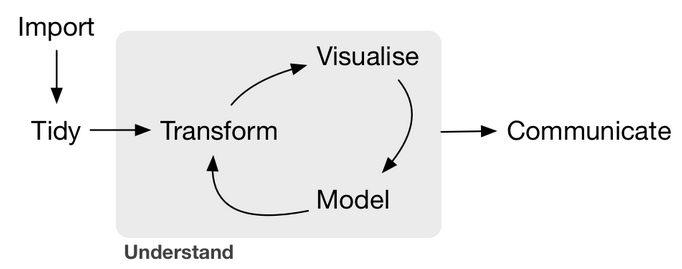
\includegraphics[width=0.75\textwidth]{../img/02_ciclo.png}
    \caption{Modelo de las herramientas que se necesitan en un proyecto de datos según \textcite[Introducción]{grolemund2016r}.}
    \label{fig:ciclo}
\end{figure}

Primero es necesario \textbf{importar} nuestros datos a R. Los datos
pueden estar en una gran cantidad de formatos o lugares.

Después, normalmente es necesario \textbf{arreglar} nuestros datos, es
decir, seguir criterios de datos limpios de manera que la manera en la
que guardemos los datos equivalga a la semántica de los datos que
tenemos. Es muy importante primero limpiar porque esto provee de
consistencia a lo largo del análisis.

Posteriormente, en casi todo proyecto, será necesario
\textbf{transformar} los datos. A veces esto implica enfocarse en un
subconjunto de los datos, generar nuevas variables, calcular
estadísticos, arreglar los datos de cierta manera, entre muchos otros.

Solamente después de estas etapas podemos empezar a generar conocimiento
a partir de los datos. Para esto tenemos dos herramientas fundamentales:
la estadística descriptiva (en el diagrama reducido a
\textbf{visualización}) y la generación de \textbf{modelos}. La primera
es fundamental pues permite derivar preguntas pertinentes a los datos,
encontrar patrones, respuestas, plantear hipótesis. Sin embargo, éstas
no escalan de la misma manera que los modelos pues estos, una vez que
aceptamos sus supuestos generan los resultados que esperamos o contestan
la pregunta planteada.

Por último, necestamos \textbf{comunicar} los resultados.

\section{Datos limpios}\label{datos-limpios}

Mucho del esfuerzo en analítica lidia con la limpieza de datos. Tomar
datos de diferentes fuentes y poderlas poner en la forma en la que uno
los necesita para realizar analítica toma mucho tiempo y esfuezo.
Existen herramientas que permiten que esta parte sea más fácil y
eficiente. Entre éstas se encuentran los criterios de datos limpios.

Los conjuntos de datos limpios (\emph{tidy datasets}) permiten
manipularlos fácilmente, modelarlos y visualizarlos. Además, tienen una
estructura específica: cada variable es una columna, cada observación
una fila y cada tipo de unidad observacional es una tabla.

\subsection{Preparación de datos}\label{preparacion-de-datos}

Esta actividad incluye una gran cantidad de elementos: desde revisar los
outliers, hasta extraer variables de cadenas en datos no estrucutrados,
imputación de valores perdidos. Los datos limpios son tan solo un
subconjunto de este proceso y lidian como el cómo estructurar los datos
de manera que se facilite el análisis.

El estándar de datos limpios está diseñado para facilitar la exploración
inicial y el análisis de datos así como simplificar el desarrollo de
herramientas para el análsis de datos que trabajen bien con datos
limpios.

Los criterios de datos limpios están muy relacionados a los de las bases
de datos relacionales y, por ende, al algebra relacional de Codd. Sin
embargo, se expresan y enmarcan en lenguaje que le es familiar a
estadísticos.

Básicamente, están creados para lidear con conjuntos de datos que se
encuentran en el mundo real. Los criterios de datos limpios proporcionan
un marco mental a través del cual la intuición es explícita.

\subsection{Definición de datos
limpios}\label{definicion-de-datos-limpios}

Los datos limpios proporcionan una manera estándar de ligar la
estructura de un dataset (es decir su layout físico) con su semántica
(su significado).

\subsubsection{Estructura de datos}\label{estructura-de-datos}

La mayoría de los datos estadísticos están conformados por tablas
rectangulares compuestas por filas y columnas. Las columnas casi siempre
están etiquetadas \emph{colnames} y las filas a veces lo están.

Tomamos el ejemplo de datos de la figura \ref{fig:estructura} en donde
se presentan datos de un experimento. La tabla contiene dos columas y
tres filas, ambas etiquetaadas.

\begin{figure}[h]
    \centering
    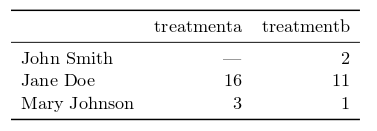
\includegraphics[width=0.4\textwidth]{../img/02_estructura.png}
    \caption{Típica presentación de datos.}
    \label{fig:estructura}
\end{figure}

Podemos estructurar los datos de diferentes manera pero la abstracción
de filas y columnas solamnete nos permite pensar en la representación
transpuesta que se muestra en la figura \ref{fig:estructurat}. El layout
cambia pero los datos son los mismos. Con columnas y filas, no podemos
decir esto de manera apropiada. Además de la simple apariencia, debemos
poder describir la semántica -el significado- de los valores que se
muestran en una tabla.

\begin{figure}[h]
    \centering
    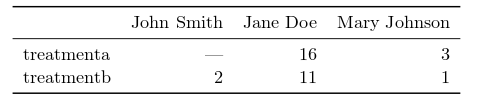
\includegraphics[width=0.5\textwidth]{../img/02_estructurat.png}
    \caption{Mismos datos que en \ref{fig:estructura} pero traspuestos.}
    \label{fig:estructurat}
\end{figure}

\subsection{Semántica}\label{semantica}

Un conjunto de datos es una colección de \textbf{valores} (normalmente
cuantitativos/números o cualitativos/caracteres).

Los valores se organian de dos maneras. Cada valor pertenece a una
variable y a una observación. Una variable contiene todos los valores de
una medida y del mismo atributo subyacente (por ejemplo, temperatura,
duración, altura, latitud) a través de unidades. Una observación, en
cambio, contiene todos los valores medidos para la misma unidad (por
ejemplo, una persona, un día, un municipio) a través de distintos
atributos.

Los mismos datos en las figuras \ref{fig:estructura} y
\ref{fig:estructurat} los pensamos ahora en estos términos. Tenemos 3
variables:

\begin{enumerate}
\def\labelenumi{\arabic{enumi}.}
\itemsep1pt\parskip0pt\parsep0pt
\item
  \emph{persona} con tres posibles valores (John, Jane, Mary)
\item
  \emph{tratamiento} con dos posibles valores (a o b)
\item
  \emph{resultado} con 5 o 6 valores (-, 16, 3, 2, 11, 1)
\end{enumerate}

El diseño del experimento mismo nos habla de la estructura de las
observaciones y los posibles valores que pueden tomar. Por ejemplo, en
este caso el valor perdido nos dice que, por diseño, se debió de
capturar esta variable pero no se hizo (por eso es importante guardarlo
como tal). Los valores perdidos estructurales, representan mediciones de
valores que no se puede hacer o que no suceden y, por tanto, se pueden
eliminar (por ejemplo, hombres embarazados). En la figura
\ref{fig:estructuratidy} se muestran los mismos datos que antes pero
pensados tal que las variables son columnas y las observaciones (en este
caso, cada punto en el diseño experimental) son filas.

\begin{figure}[h]
    \centering
    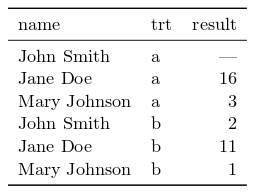
\includegraphics[width=0.4\textwidth]{../img/02_estructuratidy.png}
    \caption{Observaciones son filas, variables columnas.}
    \label{fig:estructuratidy}
\end{figure}

Normalmente, es fácil determinar qué son observaciones y qué son
variables pero es muy dificil definir en forma precisa variables y
observaciones. Por ejemplo, si tienes teléfonos de casa y celulares, se
pueden considerar como dos variables distintas en muchos contextos pero
en prevención de fraude necesitas una variable que guarde el tipo de
teléfono y otra en la que se guarde el número pues el uso regular del
mismo número de teléfono por parte de la misma persona puede ayudar a
detectarlo.

En general, es más fácil describir las relaciones funcionales entre las
variables que entre las filas (el radio, una combinación lineal).
También es más fácil hacer comparaciones entre grupos que entre columnas
(la suma, el promedio, la varianza, la moda).

\subsection{Datos limpios}\label{datos-limpios-1}

Éstos mapean de forma estándar el significado y la estructura de los
datos. Un conjunto de datos se considera sucio o limpio dependendiendo
en cómo las filas, columans y tablas mapean a observaciones, variables y
tipos. En \textbf{datos limpios}:

\begin{enumerate}
\def\labelenumi{\arabic{enumi}.}
\itemsep1pt\parskip0pt\parsep0pt
\item
  Cada \emph{variable} es una columna.
\item
  Cada \emph{observación} es una fila.
\item
  Cada \emph{tipo de unidad observacional} es una tabla.
\end{enumerate}

Esto equivale a la tercera forma normal de Codd enfocado a un solo
conjunto de datos y no a datos conectados como en bases relacionales.
Los datos sucios son cualquier otro tipo de manera de organizar los
datos.

La tabla \ref{fig:estructuratidy} corresponde a datos limpios: cada fila
es una observación, es decir, el resultado de un tratamiento a una
persona. Cada columna es una variable. Solo tenemos un tipo de unidad
observacional, es decir, cada renglón es una unidad del diseño
experimental.

Con los datos así ordenados, suele ser más fácil extraer datos que, por
ejemplo, la \ref{fig:estructura}.

\renewcommand\bcStyleTitre[1]{\large\textcolor{bbblack}{#1}}

\begin{bclogo}[
  couleur=llred,
  arrondi=0,
  logo=\bcstop,
  barre=none,
  noborder=true]{Ejercicios}
\begin{enumerate}
\item Crea un dataframe con los valores de la tabla \ref{fig:estructura} y otro 
con los valores de la tabla \ref{fig:estructuratidy}.
\item Extrae el resultado para John Smith, tratamiento a en la primera configuración y en la segunda.
\item Especifica el número de tratamientos con la forma sucia y la forma limpia.
\item Cuál es la media de los resultados: usa la forma 1 y la forma 2.
\item Extrae los tratamientos del tipo a en la forma 2.
\end{enumerate}

\end{bclogo}

Como puedes ver, los datos limpios nos permiten preguntarle cosas a los
datos de manera simple y sistemática. En particular, es una estructura
muy útil para programación vectorizada como en R (el ejercicio 5) porque
la forma se asegura que valores para diferentes variables de la misma
observación siempre están apareados.

Por convención, las variables se acomodan de una forma particular. Las
variables \emph{fijas}, en este ejemplo, las propias al diseño
experimental, van primero y posteriormente las variables \emph{medidas}.
Ordenamos éstas de forma que las que están relacionadas sean contiguas.

\section{De sucio a limpio}\label{de-sucio-a-limpio}

Los conjuntos de datos normalmente \textbf{no cumplen} con estos
criterios. Es raro obtener un conjunto de datos con el cuál podemos
trabajar de manera inmediata.

Los 5 problemas más comunes para llevar datos sucios a limpios son

\begin{enumerate}
\def\labelenumi{\arabic{enumi}.}
\itemsep1pt\parskip0pt\parsep0pt
\item
  Los nombres de las columnas son valores, no nombres de variables.
\item
  Múltiples variables se encuentran en la misma columna.
\item
  Las variables están guardadas tanto en filas como en columnas.
\item
  Muchos tipos de unidad observacional se encuentran en la misma tabla.
\item
  Una sola unidad observarcional se guardó en varias tablas.
\end{enumerate}

Estos problemas pueden ser resueltos con 3 herramientas: \emph{melting},
separación de cadenas y \emph{casting}.

\subsection{Los nombres de las columnas son valores, no nombres de
variables}\label{los-nombres-de-las-columnas-son-valores-no-nombres-de-variables}

La tabla \ref{tab:varsencols} muestra datos sucios con este problema. Se
muestran distintas religiones con el numero de personas que pertenecen a
distintos niveles de ingreso. Dentro de un reporte, este tipo de
representación tiene mucho sentido y permite visualizar muchas cosas
rápidamente.

\begin{table}[ht]
\centering
{\tiny
\begin{tabular}{lrrrrrrrrrr}
  \hline
religion & $<$\$10k & \$10-20k & \$20-30k & \$30-40k & \$40-50k & \$50-75k & \$75-100k & \$100-150k & $>$150k & Don't know/refused \\ 
  \hline
Agnostic &  27 &  34 &  60 &  81 &  76 & 137 & 122 & 109 &  84 &  96 \\ 
  Atheist &  12 &  27 &  37 &  52 &  35 &  70 &  73 &  59 &  74 &  76 \\ 
  Buddhist &  27 &  21 &  30 &  34 &  33 &  58 &  62 &  39 &  53 &  54 \\ 
  Catholic & 418 & 617 & 732 & 670 & 638 & 1116 & 949 & 792 & 633 & 1489 \\ 
  Don’t know/refused &  15 &  14 &  15 &  11 &  10 &  35 &  21 &  17 &  18 & 116 \\ 
  Evangelical Prot & 575 & 869 & 1064 & 982 & 881 & 1486 & 949 & 723 & 414 & 1529 \\ 
  Hindu &   1 &   9 &   7 &   9 &  11 &  34 &  47 &  48 &  54 &  37 \\ 
  Historically Black Prot & 228 & 244 & 236 & 238 & 197 & 223 & 131 &  81 &  78 & 339 \\ 
  Jehovah's Witness &  20 &  27 &  24 &  24 &  21 &  30 &  15 &  11 &   6 &  37 \\ 
  Jewish &  19 &  19 &  25 &  25 &  30 &  95 &  69 &  87 & 151 & 162 \\ 
  Mainline Prot & 289 & 495 & 619 & 655 & 651 & 1107 & 939 & 753 & 634 & 1328 \\ 
  Mormon &  29 &  40 &  48 &  51 &  56 & 112 &  85 &  49 &  42 &  69 \\ 
  Muslim &   6 &   7 &   9 &  10 &   9 &  23 &  16 &   8 &   6 &  22 \\ 
  Orthodox &  13 &  17 &  23 &  32 &  32 &  47 &  38 &  42 &  46 &  73 \\ 
  Other Christian &   9 &   7 &  11 &  13 &  13 &  14 &  18 &  14 &  12 &  18 \\ 
  Other Faiths &  20 &  33 &  40 &  46 &  49 &  63 &  46 &  40 &  41 &  71 \\ 
  Other World Religions &   5 &   2 &   3 &   4 &   2 &   7 &   3 &   4 &   4 &   8 \\ 
  Unaffiliated & 217 & 299 & 374 & 365 & 341 & 528 & 407 & 321 & 258 & 597 \\ 
   \hline
\end{tabular}
}
\caption{Variable de ingreso en columnas.} 
\label{tab:varsencols}
\end{table}

El conjunto de datos tiene 3 variables: \emph{religion}, \emph{ingreso}
y \emph{frecuencia}. Para arreglarlo, necesitamos \emph{juntar} (melt)
las columnas con nombres de niveles de ingreso en una sola columna que
contenga esos nombres como valores. En otras palabras, debemos convertir
de la columna 2 en adelante en filas.

Con el paquete \textbf{tidyr} esto se puede realizar en forma fácil con
el comando \texttt{gather}.

\begin{Shaded}
\begin{Highlighting}[]
\NormalTok{limpios <-}\StringTok{ }\NormalTok{tidyr::}\KeywordTok{gather}\NormalTok{(raw, }\DataTypeTok{key =} \NormalTok{income, }\DataTypeTok{value =} \NormalTok{freq, -religion)}
\end{Highlighting}
\end{Shaded}

Con este comando, obtenemos la tabla \ref{tab:ej1limpio}. Se especifica
el \emph{data.frame} como primer parámetro, la llave (parámetro
\emph{key}) será el nombre que tomará la variable con los nombres de las
columnas a juntar, el valor (parámetro \emph{value}) es el nombre de la
variable que contendrá los valores correspondientes a cada valor (la
religión i-ésima, grupo de ingreso j-ésimo) y, por último, especificamos
las variables que \textbf{NO} se deben de juntar (en este caso,
religión).

\begin{table}[ht]
\centering
\begin{tabular}{lll}
  \hline
Religion & Income & Freq \\ 
  \hline
Jewish & \$30-40k & 25 \\ 
  Mormon & \$10-20k & 40 \\ 
  Orthodox & Don't know/refused & 73 \\ 
  Other World Religions & \$30-40k & 4 \\ 
  Other Christian & \$30-40k & 13 \\ 
  Atheist & \$30-40k & 52 \\ 
  Mainline Prot & Don't know/refused & 1,328 \\ 
  Hindu & \$50-75k & 34 \\ 
  Other World Religions & \$10-20k & 2 \\ 
  Evangelical Prot & \$10-20k & 869 \\ 
   \hline
\end{tabular}
\caption{Datos limpios para religión, ingreso y frecuencia.} 
\label{tab:ej1limpio}
\end{table}

\begin{nota}[Nota] 
Esta forma es limpia pues cada columan es una variable, cada fila es una observación
y no se mezclan unidades observacionales.
\end{nota}

Este tipo de formato de datos (poner valores de variables en las
columnas) es útil también cuando se capturan datos al evitar la
repetición de valores.

Por ejemplo, pensemos en un experimento clínico en el que seguimos a
sujetos a lo largo de un tratamiento midiendo su IMC. Una forma muy
sencilla de guardar los datos del experimento es utilizando un
procesador de texto común. El capturista no querrá seguir criterios de
datos limpios al llenar la información pues implicaría repetir el nombre
de la persona, el día de la captura y el nivel de colesterol. Supongamos
un experimento con 16 sujetos a lo largo de un año en donde se mide el
colesterol una vez al mes (mes1, mes2, etc.). Los datos capturados se
muestran en la tabla \ref{tab:sujetos}.

\begin{table}[ht]
\centering
{\tiny
\begin{tabular}{llrrrrrrrrrrrr}
  \hline
sujetos & grupo & mes1 & mes2 & mes3 & mes4 & mes5 & mes6 & mes7 & mes8 & mes9 & mes10 & mes11 & mes12 \\ 
  \hline
A & control & 21.74 & 21.51 & 23.06 & 24.40 & 25.81 & 26.75 & 27.18 & 29.54 & 31.60 & 32.64 & 32.13 & 33.14 \\ 
  B & control & 20.92 & 20.90 & 21.83 & 21.85 & 24.31 & 25.62 & 24.79 & 25.34 & 26.22 & 27.81 & 29.56 & 29.72 \\ 
  C & control & 23.09 & 24.46 & 25.75 & 25.45 & 26.21 & 27.53 & 27.99 & 30.66 & 31.04 & 31.14 & 31.66 & 30.63 \\ 
  D & tratamiento & 32.44 & 34.00 & 34.21 & 33.52 & 32.73 & 32.43 & 34.35 & 35.95 & 35.67 & 37.28 & 39.09 & 39.19 \\ 
  E & tratamiento & 31.03 & 32.43 & 33.75 & 33.99 & 34.30 & 35.51 & 36.24 & 36.33 & 34.50 & 35.27 & 37.45 & 37.62 \\ 
  F & control & 16.91 & 17.05 & 16.84 & 17.49 & 18.04 & 17.10 & 17.71 & 17.30 & 19.09 & 20.83 & 21.55 & 20.99 \\ 
  G & control & 30.60 & 33.37 & 35.63 & 37.26 & 38.07 & 38.99 & 39.32 & 39.40 & 40.50 & 39.39 & 39.97 & 40.44 \\ 
  H & control & 26.37 & 26.27 & 27.61 & 27.87 & 27.46 & 26.49 & 27.65 & 27.52 & 27.98 & 29.62 & 29.61 & 30.08 \\ 
  I & tratamiento & 26.41 & 25.73 & 26.21 & 25.91 & 26.55 & 26.62 & 28.56 & 30.16 & 29.33 & 29.54 & 31.25 & 30.11 \\ 
  J & tratamiento & 34.10 & 33.29 & 34.64 & 35.43 & 35.29 & 34.15 & 35.16 & 36.73 & 36.77 & 38.43 & 38.74 & 38.71 \\ 
  K & control & 26.33 & 27.55 & 28.51 & 29.31 & 30.04 & 29.90 & 30.76 & 32.62 & 32.98 & 32.44 & 32.85 & 33.45 \\ 
  L & tratamiento & 24.58 & 26.10 & 27.76 & 28.05 & 29.45 & 30.95 & 31.90 & 32.73 & 33.77 & 34.09 & 35.50 & 35.67 \\ 
  M & tratamiento & 22.77 & 23.83 & 23.13 & 21.55 & 22.07 & 23.57 & 22.00 & 20.89 & 21.67 & 21.54 & 22.95 & 22.59 \\ 
  N & tratamiento & 32.45 & 35.28 & 34.69 & 35.37 & 35.53 & 35.64 & 35.31 & 36.32 & 36.96 & 35.46 & 34.78 & 35.83 \\ 
  O & control & 18.38 & 17.50 & 18.11 & 18.17 & 18.41 & 18.62 & 17.54 & 17.18 & 19.00 & 20.86 & 23.57 & 23.83 \\ 
  P & control & 31.64 & 32.62 & 32.55 & 30.61 & 29.65 & 32.44 & 32.93 & 35.36 & 36.51 & 38.63 & 40.48 & 39.80 \\ 
   \hline
\end{tabular}
}
\caption{Mediciones de IMC en sujetos.} 
\label{tab:sujetos}
\end{table}

\textbf{Ejercicio}

Nuevamente, queremos convertir la columan 3 a 14 en filas, es decir,
observaciones. Utiliza el comando \texttt{gather} para realizar esto y
obtener el resultado que se muestra en la tabla \ref{tab:sujetostidy}.

\begin{table}[ht]
\centering
\begin{tabular}{lllr}
  \hline
sujetos & grupo & mes & IMC \\ 
  \hline
G & control & mes8 & 39.40 \\ 
  B & control & mes9 & 26.22 \\ 
  C & control & mes8 & 30.66 \\ 
  P & control & mes1 & 31.64 \\ 
  D & tratamiento & mes7 & 34.35 \\ 
  K & control & mes6 & 29.90 \\ 
  F & control & mes1 & 16.91 \\ 
  M & tratamiento & mes6 & 23.57 \\ 
  O & control & mes11 & 23.57 \\ 
  G & control & mes7 & 39.32 \\ 
   \hline
\end{tabular}
\caption{Muestra de datos limpios para experimentos IMC.} 
\label{tab:sujetostidy}
\end{table}

\subsection{Múltiples variables se encuentran en la misma
columna}\label{multiples-variables-se-encuentran-en-la-misma-columna}

Otra forma de datos sucios es cuando una columna con nombres de
variables tiene realmente varias variables dentro del nombre (como en el
ejemplo siguiente).

\begin{table}[ht]
\centering
\begin{tabular}{lrrrrrrrrrr}
  \hline
country & year & m014 & m1524 & m2534 & m3544 & m4554 & m5564 & m65 & mu & f014 \\ 
  \hline
AD & 2000 &   0 &   0 &   1 &   0 &   0 &   0 &   0 &  &  \\ 
  AE & 2000 &   2 &   4 &   4 &   6 &   5 &  12 &  10 &  &   3 \\ 
  AF & 2000 &  52 & 228 & 183 & 149 & 129 &  94 &  80 &  &  93 \\ 
  AG & 2000 &   0 &   0 &   0 &   0 &   0 &   0 &   1 &  &   1 \\ 
  AL & 2000 &   2 &  19 &  21 &  14 &  24 &  19 &  16 &  &   3 \\ 
  AM & 2000 &   2 & 152 & 130 & 131 &  63 &  26 &  21 &  &   1 \\ 
  AN & 2000 &   0 &   0 &   1 &   2 &   0 &   0 &   0 &  &   0 \\ 
  AO & 2000 & 186 & 999 & 1003 & 912 & 482 & 312 & 194 &  & 247 \\ 
  AR & 2000 &  97 & 278 & 594 & 402 & 419 & 368 & 330 &  & 121 \\ 
  AS & 2000 &  &  &  &  &   1 &   1 &  &  &  \\ 
   \hline
\end{tabular}
\end{table}

El primer paso es pasar las columnas que son valores de variable a una
sola columna (tabla \ref{tab:tbjuntar}).

\begin{table}[ht]
\centering
\begin{tabular}{lrlr}
  \hline
country & year & column & cases \\ 
  \hline
AD & 2000 & m014 &   0 \\ 
  AE & 2000 & m014 &   2 \\ 
  AF & 2000 & m014 &  52 \\ 
  AG & 2000 & m014 &   0 \\ 
  AL & 2000 & m014 &   2 \\ 
  AM & 2000 & m014 &   2 \\ 
  AN & 2000 & m014 &   0 \\ 
  AO & 2000 & m014 & 186 \\ 
  AR & 2000 & m014 &  97 \\ 
  AS & 2000 & m014 &  \\ 
  AT & 2000 & m014 &   1 \\ 
  AU & 2000 & m014 &   3 \\ 
  AZ & 2000 & m014 &   0 \\ 
  BA & 2000 & m014 &   4 \\ 
  BB & 2000 & m014 &   0 \\ 
   \hline
\end{tabular}
\caption{Paso 1. Juntar las columnas cuyos nombres son 2 variables.} 
\label{tab:tbjuntar}
\end{table}

Posteriormente, debemos separar en las columnas apropiadas las variables
que estan contenidas en los antiguos nombres de variables (tabla
\ref{tab:tbseparar}).

\begin{table}[ht]
\centering
\begin{tabular}{lrllr}
  \hline
country & year & sex & age & cases \\ 
  \hline
AD & 2000 & m & 0-14 &   0 \\ 
  AE & 2000 & m & 0-14 &   2 \\ 
  AF & 2000 & m & 0-14 &  52 \\ 
  AG & 2000 & m & 0-14 &   0 \\ 
  AL & 2000 & m & 0-14 &   2 \\ 
  AM & 2000 & m & 0-14 &   2 \\ 
  AN & 2000 & m & 0-14 &   0 \\ 
  AO & 2000 & m & 0-14 & 186 \\ 
  AR & 2000 & m & 0-14 &  97 \\ 
  AS & 2000 & m & 0-14 &  \\ 
  AT & 2000 & m & 0-14 &   1 \\ 
  AU & 2000 & m & 0-14 &   3 \\ 
  AZ & 2000 & m & 0-14 &   0 \\ 
  BA & 2000 & m & 0-14 &   4 \\ 
  BB & 2000 & m & 0-14 &   0 \\ 
   \hline
\end{tabular}
\caption{Paso 2. Separar las columnas.} 
\label{tab:tbseparar}
\end{table}

\begin{nota}[stringr]
Otro paquete muy útil para realizar tareas de limpieza con cadenas. 
La \href{https://cran.r-project.org/web/packages/stringr/stringr.pdf}{documentación}
detalla todas sus funciones.
\end{nota}

\subsection{Las variables están guardadas tanto en filas como en
columnas}\label{las-variables-estan-guardadas-tanto-en-filas-como-en-columnas}

El problema más difícil es cuando las variables están tanto en filas
como en columnas. Para ejemplificar este problema, se muestran los datos
de temperatura máxima y mínima en algunas zonas de México.

\begin{table}[ht]
\centering
{\tiny
\begin{tabular}{lrrlrrrrrrrrrrr}
  \hline
id & year & month & element & d1 & d2 & d3 & d4 & d5 & d6 & d7 & d8 & d9 & d10 & d11 \\ 
  \hline
MX17004 & 2010 &   1 & tmax &  &  &  &  &  &  &  &  &  &  &  \\ 
  MX17004 & 2010 &   1 & tmin &  &  &  &  &  &  &  &  &  &  &  \\ 
  MX17004 & 2010 &   2 & tmax &  & 27.30 & 24.10 &  &  &  &  &  &  &  & 29.70 \\ 
  MX17004 & 2010 &   2 & tmin &  & 14.40 & 14.40 &  &  &  &  &  &  &  & 13.40 \\ 
  MX17004 & 2010 &   3 & tmax &  &  &  &  & 32.10 &  &  &  &  & 34.50 &  \\ 
  MX17004 & 2010 &   3 & tmin &  &  &  &  & 14.20 &  &  &  &  & 16.80 &  \\ 
  MX17004 & 2010 &   4 & tmax &  &  &  &  &  &  &  &  &  &  &  \\ 
  MX17004 & 2010 &   4 & tmin &  &  &  &  &  &  &  &  &  &  &  \\ 
  MX17004 & 2010 &   5 & tmax &  &  &  &  &  &  &  &  &  &  &  \\ 
  MX17004 & 2010 &   5 & tmin &  &  &  &  &  &  &  &  &  &  &  \\ 
  MX17004 & 2010 &   6 & tmax &  &  &  &  &  &  &  &  &  &  &  \\ 
  MX17004 & 2010 &   6 & tmin &  &  &  &  &  &  &  &  &  &  &  \\ 
  MX17004 & 2010 &   7 & tmax &  &  & 28.60 &  &  &  &  &  &  &  &  \\ 
  MX17004 & 2010 &   7 & tmin &  &  & 17.50 &  &  &  &  &  &  &  &  \\ 
  MX17004 & 2010 &   8 & tmax &  &  &  &  & 29.60 &  &  & 29.00 &  &  &  \\ 
  MX17004 & 2010 &   8 & tmin &  &  &  &  & 15.80 &  &  & 17.30 &  &  &  \\ 
  MX17004 & 2010 &  10 & tmax &  &  &  &  & 27.00 &  & 28.10 &  &  &  &  \\ 
  MX17004 & 2010 &  10 & tmin &  &  &  &  & 14.00 &  & 12.90 &  &  &  &  \\ 
  MX17004 & 2010 &  11 & tmax &  & 31.30 &  & 27.20 & 26.30 &  &  &  &  &  &  \\ 
  MX17004 & 2010 &  11 & tmin &  & 16.30 &  & 12.00 & 7.90 &  &  &  &  &  &  \\ 
  MX17004 & 2010 &  12 & tmax & 29.90 &  &  &  &  & 27.80 &  &  &  &  &  \\ 
  MX17004 & 2010 &  12 & tmin & 13.80 &  &  &  &  & 10.50 &  &  &  &  &  \\ 
   \hline
\end{tabular}
}
\caption{Mediciones de temperatura max y min.} 
\label{tab:clima}
\end{table}

Para limpiar, lo primero que debemos hacer es juntar los dias (que son
valores de la variable dia) en una sola columna. Después utilizamos la
nueva variable para crear la fecha. Asi, obtenemos la tabla
\ref{tab:clima1}.

\begin{Shaded}
\begin{Highlighting}[]
\CommentTok{# Tidy}
\CommentTok{# Primero, juntamos la variable dias}
\NormalTok{clean1 <-}\StringTok{ }\NormalTok{tidyr::}\KeywordTok{gather}\NormalTok{(raw, }\DataTypeTok{key =} \NormalTok{variable, }\DataTypeTok{value =} \NormalTok{value, d1:d31, }\DataTypeTok{na.rm =} \NormalTok{T)}
\NormalTok{clean1$day <-}\StringTok{ }\KeywordTok{as.integer}\NormalTok{(}\KeywordTok{str_replace}\NormalTok{(clean1$variable, }\StringTok{"d"}\NormalTok{, }\StringTok{""}\NormalTok{))}
\NormalTok{clean1$date <-}\StringTok{ }\KeywordTok{as.Date}\NormalTok{(}\KeywordTok{ISOdate}\NormalTok{(clean1$year, clean1$month, clean1$day))}
\NormalTok{clean1 <-}\StringTok{ }\NormalTok{dplyr::}\KeywordTok{select_}\NormalTok{(clean1, }\StringTok{"id"}\NormalTok{, }\StringTok{"date"}\NormalTok{, }\StringTok{"element"}\NormalTok{, }\StringTok{"value"}\NormalTok{) %>%}
\StringTok{  }\NormalTok{dplyr::}\KeywordTok{arrange}\NormalTok{(clean1, date, element) }
\end{Highlighting}
\end{Shaded}

\begin{verbatim}
## Warning in formatC(x = structure(c(14642, 14643, 14642, 14643, 14915,
## 14915, : class of 'x' was discarded
\end{verbatim}

\begin{table}[ht]
\centering
\begin{tabular}{lrlr}
  \hline
id & date & element & value \\ 
  \hline
MX17004 & 14642.00 & tmax & 27.30 \\ 
  MX17004 & 14643.00 & tmax & 24.10 \\ 
  MX17004 & 14642.00 & tmin & 14.40 \\ 
  MX17004 & 14643.00 & tmin & 14.40 \\ 
  MX17004 & 14915.00 & tmax & 31.30 \\ 
  MX17004 & 14915.00 & tmin & 16.30 \\ 
  MX17004 & 14944.00 & tmax & 29.90 \\ 
  MX17004 & 14944.00 & tmin & 13.80 \\ 
   \hline
\end{tabular}
\caption{Paso 1. Juntar las columnas, limpiar dias, crear fecha.} 
\label{tab:clima1}
\end{table}

El segundo paso es transformar la variable element en dos columnas pues,
en realidad, almacena dos variables: temperatura maxima y minima.

\begin{Shaded}
\begin{Highlighting}[]
\CommentTok{# Cast: las temperaturas van a columnas}
\NormalTok{clean2 <-}\StringTok{ }\NormalTok{tidyr::}\KeywordTok{spread}\NormalTok{(clean1, }\DataTypeTok{key =} \NormalTok{element, }\DataTypeTok{value =} \NormalTok{value)}
\end{Highlighting}
\end{Shaded}

\begin{verbatim}
## Warning in formatC(x = structure(c(14642, 14643, 14642, 14643, 14915,
## 14915, : class of 'x' was discarded
\end{verbatim}

\begin{table}[ht]
\centering
\begin{tabular}{lrlr}
  \hline
id & date & element & value \\ 
  \hline
MX17004 & 14642.00 & tmax & 27.30 \\ 
  MX17004 & 14643.00 & tmax & 24.10 \\ 
  MX17004 & 14642.00 & tmin & 14.40 \\ 
  MX17004 & 14643.00 & tmin & 14.40 \\ 
  MX17004 & 14915.00 & tmax & 31.30 \\ 
  MX17004 & 14915.00 & tmin & 16.30 \\ 
  MX17004 & 14944.00 & tmax & 29.90 \\ 
  MX17004 & 14944.00 & tmin & 13.80 \\ 
   \hline
\end{tabular}
\caption{Paso 2. Enviar a columnas las mediciones de temperaturas.} 
\label{tab:clima1}
\end{table}

\subsection{Muchos tipos de unidad observacional se encuentran en la
misma
tabla}\label{muchos-tipos-de-unidad-observacional-se-encuentran-en-la-misma-tabla}

En ocasiones las bases de datos involucran diferentes tipos de unidad
observacional. Para tener datos limpios, cada unidad observacional debe
estar almacenada en su propia tabla.

\begin{Shaded}
\begin{Highlighting}[]
\NormalTok{billboard <-}\StringTok{ }\KeywordTok{read.csv}\NormalTok{(}\StringTok{"tidyr_datasets/billboard.csv"}\NormalTok{, }\DataTypeTok{stringsAsFactors =} \NormalTok{F)}
\NormalTok{billboard_long <-}\StringTok{ }\KeywordTok{gather}\NormalTok{(billboard, week, rank, x1st.week:x76th.week, }\DataTypeTok{na.rm =} \OtherTok{TRUE}\NormalTok{)}
\NormalTok{billboard_tidy <-}\StringTok{ }\NormalTok{billboard_long %>%}
\StringTok{  }\KeywordTok{mutate}\NormalTok{(}
    \DataTypeTok{week =} \KeywordTok{extract_numeric}\NormalTok{(week),}
    \DataTypeTok{date =} \KeywordTok{as.Date}\NormalTok{(date.entered) +}\StringTok{ }\DecValTok{7} \NormalTok{*}\StringTok{ }\NormalTok{(week -}\StringTok{ }\DecValTok{1}\NormalTok{)) %>%}
\StringTok{    }\KeywordTok{select}\NormalTok{(-date.entered)}
\KeywordTok{head}\NormalTok{(billboard_tidy)}
\end{Highlighting}
\end{Shaded}

\begin{verbatim}
##   year     artist.inverted                                 track time
## 1 2000     Destiny's Child              Independent Women Part I 3:38
## 2 2000             Santana                          Maria, Maria 4:18
## 3 2000       Savage Garden                    I Knew I Loved You 4:07
## 4 2000             Madonna                                 Music 3:45
## 5 2000 Aguilera, Christina Come On Over Baby (All I Want Is You) 3:38
## 6 2000               Janet                 Doesn't Really Matter 4:17
##   genre date.peaked week rank       date
## 1  Rock  2000-11-18    1   78 2000-09-23
## 2  Rock  2000-04-08    1   15 2000-02-12
## 3  Rock  2000-01-29    1   71 1999-10-23
## 4  Rock  2000-09-16    1   41 2000-08-12
## 5  Rock  2000-10-14    1   57 2000-08-05
## 6  Rock  2000-08-26    1   59 2000-06-17
\end{verbatim}

¿Cuáles son las unidades observacionales en esta tabla?

Separemos esta base de datos en dos: la tabla canción que almacena
artista, nombre de la canción y duración; la tabla rango que almacena el
ranking de la canción en cada semana.

\begin{Shaded}
\begin{Highlighting}[]
\NormalTok{cancion <-}\StringTok{ }\NormalTok{billboard_tidy %>%}\StringTok{ }
\StringTok{  }\KeywordTok{select}\NormalTok{(artist.inverted, track, year, time) %>%}
\StringTok{  }\KeywordTok{unique}\NormalTok{() %>%}
\StringTok{  }\KeywordTok{arrange}\NormalTok{(artist.inverted) %>%}
\StringTok{  }\KeywordTok{mutate}\NormalTok{(}\DataTypeTok{song_id =} \KeywordTok{row_number}\NormalTok{(artist.inverted))}

\KeywordTok{head}\NormalTok{(cancion)}
\end{Highlighting}
\end{Shaded}

\begin{verbatim}
##   artist.inverted
## 1           2 Pac
## 2         2Ge+her
## 3    3 Doors Down
## 4    3 Doors Down
## 5        504 Boyz
## 6          98\xa1
##                                                          track year time
## 1                          Baby Don't Cry (Keep Ya Head Up II) 2000 4:22
## 2 The Hardest Part Of Breaking Up (Is Getting Back Your Stuff) 2000 3:15
## 3                                                   Kryptonite 2000 3:53
## 4                                                        Loser 2000 4:24
## 5                                                Wobble Wobble 2000 3:35
## 6                           Give Me Just One Night (Una Noche) 2000 3:24
##   song_id
## 1       1
## 2       2
## 3       3
## 4       4
## 5       5
## 6       6
\end{verbatim}

\begin{Shaded}
\begin{Highlighting}[]
\NormalTok{rango <-}\StringTok{ }\NormalTok{billboard_tidy %>%}
\StringTok{  }\KeywordTok{left_join}\NormalTok{(cancion, }\KeywordTok{c}\NormalTok{(}\StringTok{"artist.inverted"}\NormalTok{, }\StringTok{"track"}\NormalTok{, }\StringTok{"year"}\NormalTok{, }\StringTok{"time"}\NormalTok{)) %>%}
\StringTok{  }\KeywordTok{select}\NormalTok{(song_id, date, week, rank) %>%}
\StringTok{  }\KeywordTok{arrange}\NormalTok{(song_id, date) %>%}
\StringTok{  }\NormalTok{tbl_df}
\NormalTok{rango}
\end{Highlighting}
\end{Shaded}

\begin{verbatim}
## Source: local data frame [5,307 x 4]
## 
##    song_id       date  week  rank
##      (int)     (date) (dbl) (int)
## 1        1 2000-02-26     1    87
## 2        1 2000-03-04     2    82
## 3        1 2000-03-11     3    72
## 4        1 2000-03-18     4    77
## 5        1 2000-03-25     5    87
## 6        1 2000-04-01     6    94
## 7        1 2000-04-08     7    99
## 8        2 2000-09-02     1    91
## 9        2 2000-09-09     2    87
## 10       2 2000-09-16     3    92
## ..     ...        ...   ...   ...
\end{verbatim}

\subsection{Una sola unidad observarcional se guardó en varias
tablas}\label{una-sola-unidad-observarcional-se-guardo-en-varias-tablas}

Este ejemplo y datos se toman de
\url{https://dl.dropboxusercontent.com/u/1351973/tutoriales/intro_r_2.html}.

Es común que los valores sobre una misma unidad observacional estén
separados en varios archivos. Muchas veces, cada archivo es una
variable, e.g.~el mes o el nombre del paciente, etc. Para limpiar estos
datos debemos:

\begin{enumerate}
\def\labelenumi{\arabic{enumi}.}
\itemsep1pt\parskip0pt\parsep0pt
\item
  Leemos los archivos en una lista de tablas.
\item
  Para cada tabla agregamos una columna que registra el nombre del
  archivo original.
\item
  Combinamos las tablas en un solo data frame.
\end{enumerate}

La carpeta tidyr\_datasets/specdata contiene 332 archivos csv que
almacenan información de monitoreo de contaminación en 332 ubicaciones
de EUA. Cada archivo contiene información de una unidad de monitoreo y
el número de identificación del monitor es el nombre del archivo.

Primero creamos un vector con los nombres de los archivos en un
directoriocon extension .csv.

\begin{Shaded}
\begin{Highlighting}[]
\NormalTok{paths <-}\StringTok{ }\KeywordTok{dir}\NormalTok{(}\StringTok{"tidyr_datasets/specdata"}\NormalTok{, }\DataTypeTok{pattern =} \StringTok{"}\CharTok{\textbackslash{}\textbackslash{}}\StringTok{.csv$"}\NormalTok{, }\DataTypeTok{full.names =} \OtherTok{TRUE}\NormalTok{)}
\KeywordTok{names}\NormalTok{(paths) <-}\StringTok{ }\KeywordTok{basename}\NormalTok{(paths)}
\NormalTok{specdata_US <-}\StringTok{ }\KeywordTok{tbl_df}\NormalTok{(}\KeywordTok{ldply}\NormalTok{(paths, read.csv, }\DataTypeTok{stringsAsFactors =} \OtherTok{FALSE}\NormalTok{))}
\NormalTok{specdata_US}
\end{Highlighting}
\end{Shaded}

\begin{verbatim}
## Source: local data frame [772,087 x 5]
## 
##        .id       Date sulfate nitrate    ID
##      (chr)      (chr)   (dbl)   (dbl) (int)
## 1  001.csv 2003-01-01      NA      NA     1
## 2  001.csv 2003-01-02      NA      NA     1
## 3  001.csv 2003-01-03      NA      NA     1
## 4  001.csv 2003-01-04      NA      NA     1
## 5  001.csv 2003-01-05      NA      NA     1
## 6  001.csv 2003-01-06      NA      NA     1
## 7  001.csv 2003-01-07      NA      NA     1
## 8  001.csv 2003-01-08      NA      NA     1
## 9  001.csv 2003-01-09      NA      NA     1
## 10 001.csv 2003-01-10      NA      NA     1
## ..     ...        ...     ...     ...   ...
\end{verbatim}

Las variables quedaron un poco sucias\ldots{} las limpiamos y
seleccionamos solo las de interes.

\begin{Shaded}
\begin{Highlighting}[]
\NormalTok{specdata <-}\StringTok{ }\NormalTok{specdata_US %>%}
\StringTok{  }\KeywordTok{mutate}\NormalTok{(}
    \DataTypeTok{monitor =} \KeywordTok{extract_numeric}\NormalTok{(.id),}
    \DataTypeTok{date =} \KeywordTok{as.Date}\NormalTok{(Date)) %>%}
\StringTok{    }\KeywordTok{select}\NormalTok{(}\DataTypeTok{id =} \NormalTok{ID, monitor, date, sulfate, nitrate)}
\NormalTok{specdata}
\end{Highlighting}
\end{Shaded}

\begin{verbatim}
## Source: local data frame [772,087 x 5]
## 
##       id monitor       date sulfate nitrate
##    (int)   (dbl)     (date)   (dbl)   (dbl)
## 1      1       1 2003-01-01      NA      NA
## 2      1       1 2003-01-02      NA      NA
## 3      1       1 2003-01-03      NA      NA
## 4      1       1 2003-01-04      NA      NA
## 5      1       1 2003-01-05      NA      NA
## 6      1       1 2003-01-06      NA      NA
## 7      1       1 2003-01-07      NA      NA
## 8      1       1 2003-01-08      NA      NA
## 9      1       1 2003-01-09      NA      NA
## 10     1       1 2003-01-10      NA      NA
## ..   ...     ...        ...     ...     ...
\end{verbatim}

\end{document}
